\documentclass[class={myRUCProject}, crop=false]{standalone}
\IfStandalone{%
    \usepackage[disable]{todonotes}
    \import{../}{customCommands}
    \import{../}{INP-00-glossary}
    }{}
    
\begin{document}

\begin{figure}
    \centering
\begin{subfigure}{0.85\textwidth}
    \centering
    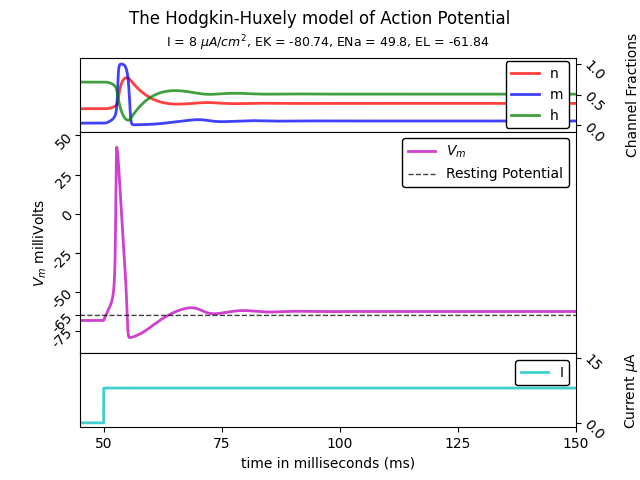
\includegraphics[width = 0.95\textwidth]{Pictures/HodHuxCurr8.png}
    \caption{}\label{fig:I08}
\end{subfigure}\\
\begin{subfigure}{0.85\textwidth}
    \centering
    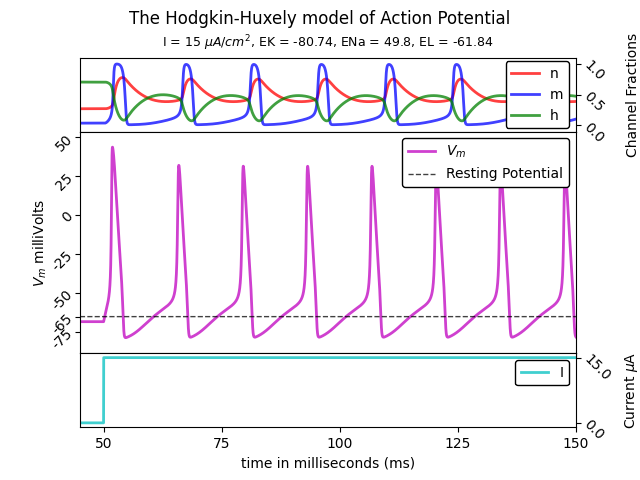
\includegraphics[width = 0.95\textwidth]{Pictures/HodHuxCurr15.png}
    \caption{}\label{fig:I15}
\end{subfigure}
\caption{All parameters of the two visible plots are identical excluding the current being fed, \labelcref{fig:I08} displays a single \gls{ap} spike in response to the current before settling, in contrast, \labelcref{fig:I15} causes a continuous cycling of of \gls{ap} spikes.}
\end{figure}

Our thorough research around the Hodgkin-Huxley model led to an efficient interpretation into coding, more specifically Python. By graphing the system we gained valid insights about the visual representations of the action potential using biophysically valid numerical variables. Just like the information we learned during our studies, our graph presents the change of the Voltage over time. Starting off with a charge of around -65mV before the action potential is activated and reaching almost +50mV and eventually returning to the resting potential, roughly at -65mV again.

The graphical representation of the coupling between our model and the Hodgkin-Huxley model can be seen in \Cref{fig:fuck}. 
\begin{figure}
    \centering
    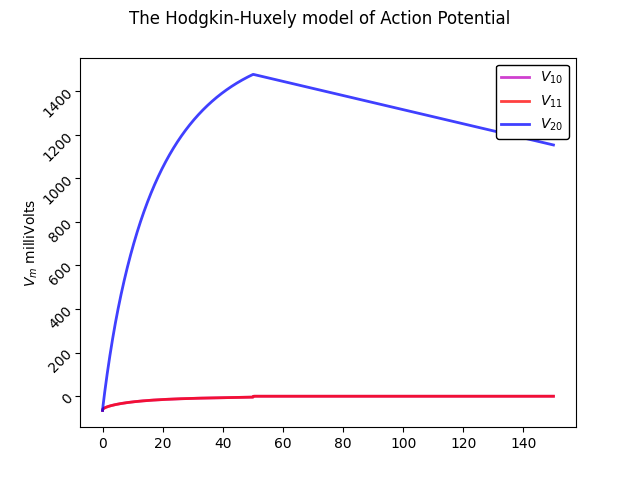
\includegraphics[trim=0 25 0 25,clip,width = 0.95\textwidth]{Pictures/Fuck.png}
    \caption{Representation of the movement of potential within the coupled model.}\label{fig:fuck}
\end{figure}
While the authors were unable to fine-tune the creation, this graph shows a proof of concept.

\end{document}